\graphicspath{{../figures/}}

\newenvironment{Messtabelle}[1]
{\begin{minipage}{\linewidth} \centering  \begin{tabular}{#1} }
{\end{tabular} \vspace*{1em} \end{minipage}} 

\section{Turingmaschinen}

\begin{frame}{Sprachen mal wieder...}
	Wir haben gesehen: Kontextfreie Grammatiken können mehr als endliche Automaten (Klammerausdrücke!).\\
	Wir wollen daher ein passendes Berechnungsmodell, das ebenfalls \enquote{mehr \nolinebreak kann} als endliche Automaten.\\
	
	\medskip
	\pause
	Wie wäre es mit einem Smartphone?\\
	Das kann ja wohl offensichtlich gültige Klammerausdrücke erkennen.\\
	\pause
	Als theoretisches Modell aber ungeeignet, da viel zu komplex.\\
	\bigskip
	Einfacheres Modell: Die \textbf{Turingmaschine}
\end{frame}

\begin{frame}{Alan Turing}
	\centering
	\vspace{-25pt}
	
\includegraphics[scale=0.35]{turing/imitationGame}
\end{frame}

\subsection{Inhalt}
\begin{frame}{Turingmaschine}
	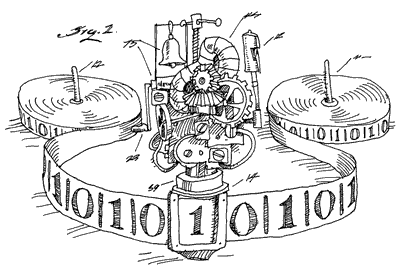
\includegraphics[scale=1]{turing/tmAufbau}
\end{frame}

\begin{frame}{Turingmaschine}
	Eine Turingmaschine besteht aus...
	\begin{itemize}[<+->]
		\item einem unendlichen Band mit einzelnen Zellen, in denen jeweils genau ein Symbol aus dem Bandalphabet steht
		\item einem Schreib-/Lesekopf, der auf genau einer Bandzelle steht
		\item einer Steuerungseinheit (Mealy-Automat), die sich in genau einem Zustand befindet
	\end{itemize}
\end{frame}

\begin{frame}{Funktionsweise der TM}
	In jedem Ausführungsschritt:
	\begin{itemize}[<+->]
		\item TM liest das Symbol, auf dem der Kopf steht
		\item Steuerung entscheidet über die Ausgabe, den Folgezustand und die Bewegung
		\item Ausgabe wird an der aktuellen Position auf das Band geschrieben
		\item Steuerung wechselt in den Folgezustand
		\item Kopf bewegt sich einen Schritt nach links oder rechts oder bleibt stehen
	\end{itemize}
	\pause
	Die TM hält, wenn für einen Zustand und das gelesene Symbol keine Übergänge in der Steuerung definiert sind. \textbf{Eine TM muss nicht halten!}
\end{frame}

\begin{frame}{Ein-/Ausgabe}
	\begin{block}{Eingabe}
		Am Anfang steht das Eingabewort umgeben von Blanksymbolen auf dem Band, der Kopf steht auf dem ersten Zeichen des Eingabeworts.
	\end{block}
	\pause
	
	\begin{block}{Ausgabe}
		Zwei Möglichkeiten:
		\begin{itemize}[<+->]
			\item Berechnung von Funktionen: Ausgabewort steht am Ende auf dem Band
			\item Erkennen von Sprachen: Halten in akzeptierendem Zustand\\
				  Wir bezeichnen dann wieder mit $L(T)$ die akzeptierte Sprache
		\end{itemize}
	\end{block}
\end{frame}


\begin{frame}{Beispiel}
	\vspace{-30pt}
	    \begin{center}

			\begin{tikzpicture}[shorten >=1pt,initial text=,node distance=2cm,auto,->,>=stealth,baseline=(B.base)]
			% \node[state,initial]  (S)                       {$S$};
			\node[state,initial]  (A)          {$A$};
			% \node (nix) [right of=A] {};
			\node[state]          (B) [above right of=A] {$B$};
			\node[state]          (C) [right of=B] {$C$};
			\node[state]          (E) [below right of=A] {$E$};
			\node[state]          (D) [right of=E] {$D$};
			\path[->]
			% (S) edge              node  {$\9\io\9R$} (A)
			(A) edge              node  {$\#1\io\#XR$} (B)
			(B) edge [loop above] node  {$\#1\io\#1R$} ()
			edge              node  {$\9\io\9R$} (C)
			(C) edge [loop above] node  {$\#1\io\#1R$} ()
			edge              node  {$\9\io\#1L$} (D)
			(D) edge [loop below] node  {$\#1\io\#1L$} ()
			edge              node  {$\9\io\9L$} (E)
			(E) edge [loop below] node  {$\#1\io\#1L$} ()
			edge              node  {$\#X\io\#1R$} (A)
			% (B) edge              node        {$\9\io\9R$} (B)
			% edge [loop right] node        {$\#1\io\#1R$} ()
			% (B) edge [loop right] node {$\9\io\#1L$} ()
			% edge  node [pos=0.3]       {$\#1\io\#1L$} (A)
			;
			\end{tikzpicture}
			\bigskip

			\begin{tabular}{c|c|c|c|c|c}
				& A & B & C & D & E \\ \hline
				$\square $ & & C,$\square$,R & D, $1$, L & E,$\square$, L & \\ \hline
				$1$ & B,$X$, R & B,$1$, R & C,$1$, R & D,$1$, L & E,$1$, L \\ \hline
				$X$ & & & & & A,$1$,R \\
			\end{tabular}
	\end{center}
\end{frame}

\begin{frame}{Beispiel}
	\only<1|handout:1>{Eingabe: $11$}
	\bigskip
	\begin{itemize}
		\only<1-3|handout:1>{\item[1] \begin{Messtabelle}{ccccccc} & A & & & & & \\ & $\downarrow$ &&&&& \\ 
				$\square$ & 1 & 1 & $\square$ & $\square$ & $\square$ & $\square$ \end{Messtabelle} }
		\only<2-4|handout:1>{\item[2] \begin{Messtabelle}{ccccccc} &  & B & & & & \\ & &$\downarrow$ &&&& \\ 
				$\square$ & X & 1 & $\square$ & $\square$ & $\square$ & $\square$ \end{Messtabelle} }
		\only<3-5|handout:1>{\item[3] \begin{Messtabelle}{ccccccc} &  & & & C& &  \\ &  &&& $\downarrow$ & &\\ 
				$\square$ & X & 1 & $\square$ & $\square$ & $\square$ & $\square$ \end{Messtabelle} }
		\only<4-6|handout:2>{\item[4] \begin{Messtabelle}{ccccccc} &  & & D & & &  \\ &  && $\downarrow$ &&& \\ 
				$\square$ & X & 1 & $\square$ & 1 & $\square$  & $\square$ \end{Messtabelle} }
		\only<5-7|handout:2>{\item[5]  \begin{Messtabelle}{ccccccc} &  & E &  & & &  \\ &  & $\downarrow$ &&&& \\ 
				$\square$ & X & 1 & $\square$ & 1 & $\square$  & $\square$ \end{Messtabelle} }
		\only<6-8|handout:2>{ \item[6] \begin{Messtabelle}{ccccccc} &  &   A && & &  \\ &  &  $\downarrow$ &&&& \\ 
				$\square$ & 1 & 1 & $\square$ & 1 & $\square$  & $\square$ \end{Messtabelle} }
		\only<7-9|handout:3>{\item[7] \begin{Messtabelle}{ccccccc} &  &    & B & & &  \\ &  &&  $\downarrow$ &&& \\ 
				$\square$ & 1 & X & $\square$ & 1 & $\square$  & $\square$ \end{Messtabelle} }
		\only<8-10|handout:3>{\item[8] \begin{Messtabelle}{ccccccc} &  &    &  & & C &  \\ &  && && $\downarrow$ & \\ 
				$\square$ & 1 & X & $\square$ & 1 & $\square$  & $\square$ \end{Messtabelle} }
		\only<9-11|handout:3>{\item[9] \begin{Messtabelle}{ccccccc} &  &    &  &  D& &  \\ &  && & $\downarrow$ && \\ 
				$\square$ & 1 & X & $\square$ & 1 & 1  & $\square$ \end{Messtabelle} }
		\only<10-12|handout:4>{\item[10] \begin{Messtabelle}{ccccccc} &  &   E &  &  & &  \\ &   & $\downarrow$ && &&\\ 
				$\square$ & 1 & X & $\square$ & 1 & 1  & $\square$ \end{Messtabelle} }
		\only<11-12|handout:4>{\item[11] \begin{Messtabelle}{ccccccc} &  &    & A &  & &  \\ &   && $\downarrow$ && &\\ 
				$\square$ & 1 & 1 & $\square$ & 1 & 1  & $\square$ \end{Messtabelle} }
	\end{itemize}
	\only<12|handout:4>{ Also allgemein : Eingabe von $1^k$ wird zu $\square \, 1^k \, \square \, 1^k \, \square $} 
\end{frame}

\begin{frame}
	\vspace{-30pt}
	\begin{figure}[H]
		\centering
		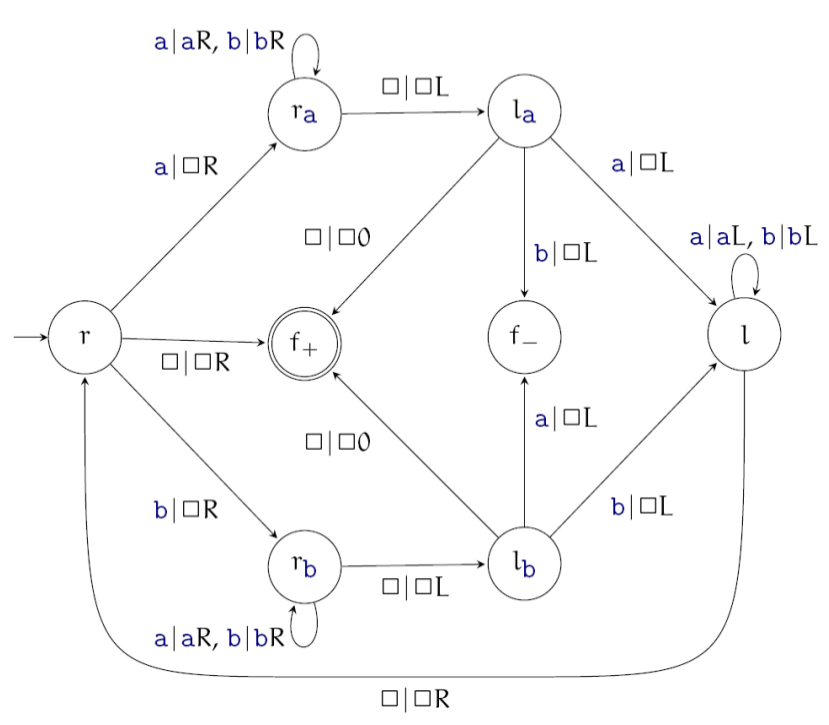
\includegraphics[scale=0.45]{turing/Palindrom}
	\end{figure}
\end{frame}

\begin{frame}{Turingmaschine}
	\begin{Definition}
		Eine Turingmaschine $T$ ist definiert als $$ T = (Z, z_0 , X, f,g, m)$$
		\begin{itemize}[<+->]
			\item $Z \quad$ Zustandsmenge 
			\item $z_0\in Z \quad$ Startzustand
			\item $X \quad$ Bandalphabet mit $\square \in X$
			\item $f:Z\times X \dashrightarrow Z \quad$ Übergangsfunktion
			\item $g:Z\times X\dashrightarrow X \quad$ Ausgabefunktion 
			\item $m:Z\times X \dashrightarrow \{\text{L},\text{N},\text{R}\} \quad$ Bewegungsfunktion
		\end{itemize}
		\pause
		Alle Funktionen können auch nur partiell definiert sein.
	\end{Definition}
\end{frame}


\begin{frame}{Konfiguration}
	\begin{Definition}
		Als \textbf{Konfiguration} $ c =(z,b,p)$ bezeichnen wir den Zustand einer Turing-Maschine zu einem Zeitpunkt. Dabei ist 
		\begin{itemize}
			\item $z\in Z$ der Zustand
			\item $b: \Z\to X$ die Bandbeschriftung
			\item $p\in \Z$ die Position des Zeigers.
		\end{itemize}
	\end{Definition}
\end{frame}

\begin{frame}{Berechnungsschritte}
	\begin{Definition}
		In einem Berechnungsschritt geht eine TM aus einer Konfiguration $c$ 
		in die Konfiguration $$\Delta_1(c) := c' = (z',b',p')$$ über, wobei gilt:
		\begin{itemize}[<+->]
			\item $z' = f(z,b(p))$
			\item $\forall i\in \Z: b'(i) =
			\begin{cases}
			b(i) & \text{ falls } i\not=p \\
			g(z,b(p)) & \text{ falls } i=p
			\end{cases}$
			\item $p' = p + m(z,b(p))$
		\end{itemize}
		\bigskip
		
		\pause
		Wenn $\Delta_1(c)$ nicht definiert ist, bezeichnet man $c$ als \textbf{Endkonfiguration} und die TM \textbf{hält}.
	\end{Definition}
\end{frame}

\begin{frame}{Berechnungen}
	\begin{Definition}
		Eine Berechnung ist eine Folge von Konfigurationen $(c_0, c_1, ..., c_t)$ bei der gilt $$c_{i+1} = \Delta_1(c_i)$$ \pause
		Es gibt endliche, haltende (endet in einer Endkonfiguration) und unendliche Berechnungen.
		\bigskip
		
		\pause
		Induktiv definiert man $\Delta_t(c) , t\in\N_0$ als die Konfiguration, welche nach $t$ Berechnungsschritten erreicht werden kann und $\Delta_*(c)$ als Endkonfiguration, die von $c$ aus erreicht wird (falls die Berechnung endet).
	\end{Definition}
\end{frame}

\begin{frame}{Aufgabe}
	Was macht die folgende Turingmaschine für Eingaben aus $\{0, 1\}^*$?
	
	\smallskip
	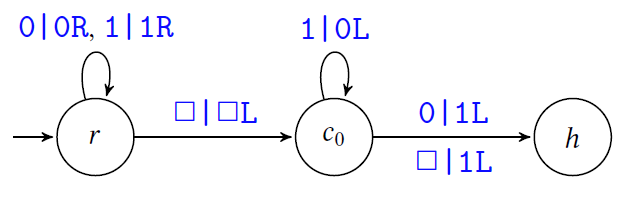
\includegraphics[scale=0.65]{turing/addBin1}
	
	\smallskip
	\visible<2|handout:2>{
		Inkrementieren der dargestellten Zahl um $1$.
	}
\end{frame}


\begin{frame}{Aufgabe}
	Entwerfen Sie eine Turingmaschine, die für eine Eingabe $w \in \{0, 1\}^*$ $$Repr_2(Num_2(w) - 1)$$ berechnet. Sie dürfen davon ausgehen, dass $Num_2(w) > 0$ gilt.\\
	\pause
	Achtung: Was passiert mit führenden Nullen?\\
	% TODO: Löung
	
	\bigskip
	Wie würde man eine (einfache, nicht effiziente) TM zum Addieren von zwei Zahlen in Binärdarstellung aufbauen?
\end{frame}


\begin{frame}{Entscheidbarkeit}
	\begin{Definition}
		Eine Sprache $L$ ist eine   
		\begin{itemize}[<+->]
			\item \textbf{aufzählbare Sprache}, wenn es eine Turingmaschine gibt, die $L$ akzeptiert.
			\item \textbf{entscheidbare Sprache}, wenn es eine Turingmasche gibt, die $L$ akzeptiert und \emph{für jede Eingabe} hält.
		\end{itemize}
	\end{Definition} \pause
	
	Bei aufzählbaren Sprachen ist nicht definiert, wie sich die TM für Wörter $ w \notin L$ verhält. Sie kann diese ablehnen oder nicht halten. Ob eine TM für eine Eingabe nicht hält, können wir \enquote{von Außen} nicht einfach feststellen.
\end{frame}


\begin{frame}{Aufgabe}
	Entwerfen Sie eine Turingmaschine, die $w\in \{0^k1^k | k\in \N_0 \} $ akzeptiert.
	% TODO Lösung
\end{frame}

\begin{frame}{Aufgabe}
	Entwirf eine TM, die alle gültigen Klammerausdrücke entscheidet.\\
	Gültige Klammerausdrücke werden dabei von der folgenden Grammatik produziert: $ G = (\{S\},\{(, )\}, S, P )$ mit den Produktionen $ S \to \eps \mid (S)S$.
\end{frame}
